\documentclass{article}
\usepackage{hyperref}
\usepackage{amsmath}
\usepackage{amsfonts}
\usepackage{amssymb}
\usepackage{graphicx}\graphicspath{{figs}{notebooks}{.}}
% \usepackage[margin=1in]{geometry}
\usepackage{comment}
\usepackage{color}

\title{Denoising in Microscopy Imaging}

\author{Vicente González-Ruiz and José Jesús Fernández Rodríguez}

\begin{document}
\maketitle

\begin{abstract}
%{{{

  We evaluate several image denoising algoritms commonly used in
  electron microscopy of biological specimens. Microscopy images are
  characterized by a very low SNR and denoising algorithms are
  required to improve their posterior analysis. It is also common that
  there exist only one noisy version of the images, which increases
  the dificulty of evaluating the algorithms (we don't have a ground
  truth to compare with) and the selection the denoising parameters.

%}}}
\end{abstract}

\tableofcontents

\section*{Definitions and notation}
%{{{

\begin{tabular}{ll}
  $x$ & A scalar value (e.g., a value of a pixel of a grayscale image) \\
  $\mathbf{X}$ & A tensor structure (e.g., an image) \\
  $\mathbf{X}_i$ & The $i$-th element of $\mathbf{X}=\{\mathbf{X}_i\}_{i=1}^N=\{\mathbf{X}_i\}$ \\
  $\hat{\mathbf{X}}^{(i)}$ & The $i$-th noisy instance of the signal $\mathbf{X}$ \\
  $\tilde{\mathbf{X}}^{[I]}$ & The mean of the noisy instances $\{\hat{\mathbf{X}}^{(i)}\}_{i=1}^I$ \\ 
  $\overline{\mathbf{X}}$ & The mean of the samples of $\mathbf{X}$ \\ 
  $\text{size}(\mathbf{X})$ & The number of elements in $\mathbf{X}$ \\
  $\text{rank}(\mathbf{X})$ & The number of dimensions in $\mathbf{X}$ \\
  %$|\mathbf{X}_i|$ & The absolute value of $\mathbf{X}_i$ \\
  $\alpha\mathbf{X}$ & $=\{\alpha\mathbf{X}_i\}$ (scalar multiplication) \\
  $\mathbf{X}+\mathbf{Y}$ & $=\{\mathbf{X}_i + \mathbf{Y}_i\}$ (Hadamard addition) \\ 
  $\mathbf{X}\mathbf{Y}$ & $=\{\mathbf{X}_i\mathbf{Y}_i\}$ (Hadamard product) \\ 
  $\mathcal{N}$ & The normal distribution \\ 
  $\mathcal{P}$ & The Poisson distribution \\
  $\mathbf{X}\sim\mathcal{N}$ & The elements of $\mathbf{X}$ follows a normal distribution \\
  $\mathbf{X}_{\mathcal{N}}$ & The same as $\mathbf{X}\sim\mathcal{N}$ \\
  $\Pr(\mathbf{X}=x)$ & Probability that a $\mathbf{X}_i$ takes the value $x$ \\
  $\Pr(\mathbf{X}=x, \mathbf{Y}=y)$ & $\Pr(\mathbf{X}=x)$ and $\Pr(\mathbf{Y}=y)$ (joint probability)  \\
  $\mathrm{Su}(\mathbf{X})$ & $=\{x\in\mathbb{R}|\Pr(\mathbf{X}=x)>0\}$ (support of $\mathbf{X}$)\\
  $\Pr(A|B)$ & Conditional probability of $A$ given $B$ \\
  $\mathbb{E}(\mathbf{X})$ & Expectation of $\mathbf{X}$ \\ 
  $A(b)$ & $A$ depends on (parameter) $b$ \\
  $\mathcal{F}$ & The (forward) Fourier transform ($\mathcal{F}(x)=X$) \\
  $\mathcal{F}^{-1}$ & The inverse Fourier transform \\
  $\mathbf{X}*\mathbf{Y}$ & $=\mathcal{F}^{-1}(\mathcal{F}(\mathbf{X})\mathcal{F}(\mathbf{Y}))$ (convolution) \\
  $A[b]$ & The sampled version of $A(b)$
\end{tabular}

%}}}

\section{Common sources of noise in microscopy imaging}
%{{{

In microscopy, there are three main sources of noise: (1) \emph{dark
  noise} which corresponds to the electronic noise generated by the
thermal agitation of electrons, (2) \emph{photon noise} (or shot
noise) that is generated by the fluctuations in the number of photons
sensed at a given signal exposure level, and (3) the \emph{readout
  noise}, generated by the non-perfectness of the output electronic
amplifiers used in the process of converting photon or electron
accumulations into voltages. Therefore, the level of noise depends on
the exposure time, experimental conditions affecting the sensors such
as the temperature, among other capturing parameters. Dark and photon
noises are modeled as a Poisson distribution $\mathcal{P}(\lambda)$, where
$\lambda$ represents the average dark flux. Readout noise is modeled
as zero-mean additive white Gaussian noise
\cite{meiniel2018denoising,zhou2020wirtinger}.

\begin{comment}
\subsection{Quantization noise}
%{{{

All digital capturing devices generate quantization noise which is
usually modeled as additive zero-mean uniform noise
(${\mathbf N}\sim{\mathcal U}(c)$). The PDF (Probability Density
Function) is defined by
\begin{equation}
  f(x; c) = \Pr({\mathbf N}^{(i)}_j{=}x) \triangleq \begin{cases}
    \frac{1}{2c} & \text{for } -c \le x \le c, \\[8pt]
    0 & \text{for } x < c \ \text{ or } \ x > -c,
  \end{cases}
\end{equation}
$x$ and $f$ continuous, where $\Pr(\cdot)$ represents the
probability of $\cdot$, and $c$ controls the amplitude of the
noise. Notice that in this case, $\overline{\mathbf{N}}^{(i)}=0$ and
therefore, $\overline{\mathbf N}={\mathbf 0}$ (see
Eq.~\ref{eq:noise_expectation_2}). 

%}}}
\end{comment}

\subsection{Zero-mean Additive White Gaussian (ZAWG) noise}
%{{{

A noisy signal $\hat{\mathbf X}$ corrupted by ZAWG noise can be modeled as
\begin{equation}
  \hat{\mathbf X} = {\mathbf X} + {\mathbf N}_{{\mathcal N}(\sigma)},
  \label{eq:AWG_noise_model}  
\end{equation}
where $\mathbf{X}$ is the \emph{clean} signal (without noise, ground
truth usually unknown),
and ${\mathbf N}$ is a tensor of random samples,
where, for the ZAWG noise case,
${\mathbf N}\sim{\mathcal N}(\mu=0,\sigma)$, with PDF (probability density
function)
\begin{equation}
  \Pr({\mathbf N}{=}x) = \frac 1 {\sigma\sqrt{2\pi}} e^{-\frac{x^2}{2\sigma^2} }.
\end{equation}
In theory, $x\in\mathbb{R}$ can be continuous, although in our
context, $x$ is a signal sample and therefore, discrete,
$\mu\in\mathbb{R}$ is the mean, and $\sigma\in\mathbb{R}$ represents
the standard deviation of the noise. Notice that this is a
signal-independent model because nothing can said about ${\mathbf N}$
known $\hat{\mathbf X}$, except that
\begin{equation}
  \Pr(\mathbf{N}{=}n|\hat{\mathbf{X}}) = \Pr(\mathbf{N}{=}n).
\end{equation}

By definition, the spectrum of AWG noise is flat. Therefore, the
performance of a pure low-pass filter denoiser will depend on the
shape of the spectrum of $\mathbf{X}$.

%}}}

\subsection{Poisson noise}
%{{{

Poisson noise is defined by the PMD (Probability Mass
Distribution)\footnote{Also called discrete PDF.}
\begin{equation}
  \Pr({\mathbf N}_j{=}k) = \frac{\mathbf{\lambda}_j^ke^{-\mathbf{\lambda}_j}}{k!},
  \label{eq:PN}
\end{equation}
which describes the probability of $k\in\mathbb{N}$ events ocurring
within an observed interval (of time, for example), when, on average
we have ${\mathbf \lambda}_j\in\mathbb{R}$ events in such interval. In
this case, we model the noisy as
\begin{equation}
  \hat{{\mathbf X}}_j = \frac{{\mathbf X}_j^{k} e^{-{\mathbf X}_j}}{k!}.
\end{equation}

As can be seen, this is a signal-dependent model because the brighter
parts of $\hat{\mathbf X}$ will have a higher mean value and a higher
variance\footnote{The mean and variance of a Poisson law are both
  equal to $\lambda$.}, and therefore a higher noise level
\cite{meiniel2018denoising}. For this reason, we model Poisson noise
with
\begin{equation}
  \hat{\mathbf{X}} = \frac{\mathbf{N}(\mathbf{X})}{\gamma},~\mathbf{N}\sim\mathcal{P}(\lambda=\gamma\mathbf{X}).
\end{equation}

Poisson noise depends on the intensity of the clean signal $\mathbf{X}$ and
therefore, the frequency characteristics of $\mathbf{N}$ resemble the
spectrum of $\mathbf{X}$.

%}}}

\subsection{Mixed Poisson-Gaussian (MPG) noise}
%{{{

A more realistic noise model in microscopy consists in a combination
of both Poisson and ZAWG noise, which is commonly called mixed
Poisson-Gaussian (MPG) noise \cite{meiniel2018denoising}. In this
case, we have that
\begin{equation}
  \Pr({\mathbf N}{=}k) = \frac{e^{-\lambda_j}}{\sqrt{2\pi}\sigma}\sum_{p=0}^{\infty}\frac{\lambda_j^p}{p!} e^{-\frac{\gamma p - k}{2\sigma^2}},
  \label{eq:PN}
\end{equation}
and that
\begin{equation}
  \hat{\mathbf X} = (1-\alpha)(\mathbf{X} + {\mathbf N}_{\mathcal{N}(\sigma)}) + \alpha{\mathbf N}_{\mathcal{P}(\lambda=\gamma\mathbf{X})}/\gamma,
  \label{eq:MPG_noise_model} 
\end{equation}
where $\alpha\in[0,~1]$ controls the ratio of both types of
noise. Therefore, for $\alpha\neq 0$,\footnote{If $\sigma=0$ and
  $\alpha=0$, the Gaussian noise vanishes and
  $\hat{\mathbf{X}}=\mathbf{X}$.}  ${\mathbf{N}}$ is signal-dependent
and it's spectrum depends on $\mathbf{X}$. By default, in our
experiments, $\alpha=0.5$.

%}}}

% \subsection{Speckle noise}
%{{{

% Speckle noise is generated in optical devices that use coherent light sources (lasers), such as in fluorescence microscopy \cite{kumar2021speckle}. Speckle noise is signal-dependent, so its variance changes with the intensity of the true image. It has been modeled as zero-mean multiplicative Gaussian noise \cite{} and as Rice noise \cite{}.

% Multiplicative zero-mean Gaussian noise, modeled as
%   \begin{equation}
%     \hat{\mathbf X}^{(i)} = {\mathbf X} (1 + {\mathbf N}^{(i)}),
%     \label{eq:MGN}
%   \end{equation}
%   where ${\mathbf N}\sim{\mathcal N}(\mu,\sigma)$. This is a signal-dependent noise present
%   in synthetic aperture radar (SAR) and ultrasound images is usually
%   considered speckle noise.
  
%   Another distribution used for modeling speckle noise is the Rice
%   distribution ($\mathbf{N}\sim\mathrm{Rice}(\nu,\sigma)$), with PDF
%   \begin{equation}
%     f(x; \nu,\sigma) = \Pr({\mathbf N}^{(i)}_j{=}x) = \frac{x}{\sigma^2}e^{\frac{-(x^2+\nu^2)}{2\sigma^2}}I_0\left(\frac{x\nu}{\sigma^2}\right),
%   \end{equation}
%   where $x$ is continuous, and $I_o$ is the modified Bessel function
%   of the first kind with order zero. Rician noisy tensor instances can
%   be generated with
%   \begin{equation}
%     \hat{\mathbf X}^{(i)} = \sqrt{ ({\mathbf X} + {\mathbf N}_{\text{real}}^{(i)})^2 + ({\mathbf N}_{\text{imag}}^{(i)})^2}.
%   \end{equation}
%   %Notice that the Rayleigh distribution ($\mathbf{N}\sim\mathrm{Rayleigh}(\sigma)$),
%   %which is defined by the PDF
%   %\begin{equation}
%   %  {\mathbf N}^{(i)} \sim f(x; \sigma) = \frac{x}{\sigma^2} e^{-x^2/(2\sigma^2)}, \quad x \geq 0,
%   %\end{equation}
%   %continuous both, $x$ and $\sigma$ (the scale parameter) is a
%   %particular case of Rice distribution when $\nu=0$.
%   Notice that, even being $\nu=0$ (in whose case we are working with
%   the Rayleigh distribution
%   ($\mathbf{N}\sim\mathrm{Rayleigh}(\sigma)$)), the mean of the noise
%   is not zero. The noise that corrupts magnetic resonance images is
%   usually modeled as Rician/Rayleigh noise.

%}}}

% \section{Noise models}
%{{{

% \label{sec:noise_models}

% Let $\mathbf{X}$ be a \emph{clean signal} (without noise, ground truth
% usually unknown) tensor, and $\hat{\mathbf X}^{(i)}$ the $i$-th
% noisy-version tensor random instance of $\mathbf{X}$ generated, in
% general, through
% \begin{equation}
%   \hat{\mathbf X}^{(i)} = f(\mathbf{X}, \mathbf{N}^{(i)}),
%   \label{eq:general_model}
% \end{equation}
% where ${\mathbf N}^{(i)}$ an $i$-th (unknown) noise tensor instance
% with the same shape as $\mathbf{X}$.

% We assume that ${\mathbf X}$ and $\mathbf{N}$ are statistically
% independent, and therefore, nothing can be said about
% ${\mathbf N}^{(i)}$ if we know $\hat{\mathbf X}^{(i)}$, and
% viceversa, and therefore, it is impossible to obtain ${\mathbf X}$
% from a single $\hat{\mathbf X}^{(i)}$.

% \subsection{Signal-independent noise model}
% In SIN (signal-independent noise) models, the noise is statistically i.i.d. (independent and
% identically distributed), i.e., the random values of ${\mathbf N}^{(i)}$ satisfy that
% \begin{equation}
%   {\mathbb E}[\{{\mathbf N}^{(i)}_j\}_{j=1}^J]=\frac{1}{J} \sum_{i=1}^J {\mathbf N}_j^{(i)}=\overline{\mathbf N}^{(i)},
%   \label{eq:noise_expectation_1}
% \end{equation}
% where ${\mathbf N}^{(i)}_j$ is the $j$-th (scalar) value
% of ${\mathbf N}^{(i)}$, and
% \begin{equation}
%   J=\prod_{k=1}^D \mathbf{X}.\text{shape}[k],
% \end{equation}
% being $D$ the number of dimensions of the signal (in microscopy, usually 2 or 3).

% SIN models are also called additive noise models defined by
% \begin{equation}
%   \hat{\mathbf X}^{(i)} = {\mathbf X} + {\mathbf N}^{(i)}.
%   \label{eq:additive_noisy_model}
% \end{equation}

% \subsection{Signal-dependent noise (SDN) models}
% In SDN models, the amplitude of the random noise samples depends on
% the clean signal (see Eq.~\ref{eq:general_model}).

% %\begin{equation}
% %  \hat{\mathbf X}^{(i)} = \mathbf{X} + {\mathbf N}^{(i)}(\mathbf{X}),
% %  \label{eq:SDN_model}
% %\end{equation}

%}}}

%}}}

\section{Distortion metrics}
%{{{

\subsection{\href{https://en.wikipedia.org/wiki/Root_mean_square_deviation}{Root Mean
    Square Error (RMSE)}}
%{{{

Having two images $\mathbf{X}$ and $\mathbf{Y}$ of size $J$,
\begin{equation}
  \text{RMSE}(\mathbf{X},\mathbf{Y}) = \sqrt{\frac{1}{J}\sum_{i=1}^J(\mathbf{X}_i - \mathbf{Y}_i)^2}.
\end{equation}
Notice that the RMSE expresses the distortion in the same units as the
samples (pixels/voxels).

%}}}

\subsection{\href{https://en.wikipedia.org/wiki/Structural_similarity_index_measure}{Structural
    Similarity Index Measure (SSIM)}}
%{{{

The SSIM try to model the human perception of the differences between
two images $\mathbf{X}$ and $\mathbf{Y}$. The metric returns a real
number between $[-1, 1]$, $-1$ representing the perfect dis-similarity
case, $0$ no similarity, and $1$ perfect similarity. The SSIM index is
determined (splitting the input images into $M$ non-overlapping blocks)
with
\begin{equation}
  \text{SSIM}(\mathbf{X}, \mathbf{Y}) = \frac{1}{J} \sum_{j=1}^J \frac{(2\overline{\mathbf{x}}_j \overline{\mathbf{y}}_j + c_1)(2\sigma_{\mathbf{x}_j \mathbf{y}_j} + c_2)}{(\overline{\mathbf{x}_j^2} + \overline{\mathbf{y}_j^2} + c_1)(\sigma^2_{\mathbf{x}_j} + \sigma^2_{\mathbf{y}_j} + c_2)},
\end{equation}
where $\overline{\mathbf x}_j$ is the mean of the $j$-th block of
$\mathbf{X}$, $\sigma^2_{\mathbf{x}_j}$ is its variance (equivalently
for $\mathbf{Y}$), $\sigma_{\mathbf{x}_j\mathbf{y}_j}$ is the
covariance of both blocks, $c_1=(k_1L)^2$, $c_2=(k_2L)^2$ are two
variables used to stabilize the division with weak denominator, $L$ is
the dynamic range of the samples, $k_1=0.01$, and $k_2=0.03$, and
where the default size of the local blocks is $7^D$, where $D$ is the
number of signal dimensions. When evaulating, SSIM values below $0$
does not make sense.

%}}}

\subsection{\href{https://en.wikipedia.org/wiki/Pearson_correlation_coefficient}{Pearson Correlation Coefficient (PPC)}}
%{{{

The PPC is given
by
\begin{equation}
  \text{PPC}(\mathbf{X}, \mathbf{Y}) = \frac{\sum_j(\mathbf{X}_j - \overline{\mathbf{X}})(\mathbf{Y}_j - \overline{\mathbf{Y}})}{\sqrt{\sum_j (\mathbf{X}_j - \overline{\mathbf{X}})^2 \sum_j (\mathbf{Y}_j - \overline{\mathbf{Y}})^2}},
\end{equation}
and measures the linear correlation between two tensors $\mathbf{X}$
and $\mathbf{Y}$.  As happen with the SSIM, the output is in
$[-1, -1]$, meaning $-1$ a perfect negative linear relationship
between the input tensors, $0$ no linear relation, and $1$ a perfect
coincidence. However, as happens with the SSIM, in microscopy values
below $0$ never should occur.

%}}}

\subsection{Fourier Shell Correlation (FSC) and Fourier Ring Correlation (FRC) curves}
%{{{

The FSC curve measures the similarity between two 3D volumes
represented in the Fourier domain \cite{verbeke2024self} (for the 2D
case, the equivalent metric is called FRC). Each point of a curve
prepresents the normalized cross-correlation between two ``shells''
(``rings'' in 2D) of Fourier coefficients of both volumes
(images). When the number of dimensions is not relevant, we will refer
to this metric simply by FC (Fourier Correlation).

An advantage of the FC over other similarity metrics such as the
RMSE, the SSIM and the PPC is that FC values depend on the frequency,
and this can be interesting in some scenarios, such as microscopy,
where the resolution of the microscope is finite and known a priori
\cite{nieuwenhuizen2013measuring}. Notice that, with this information,
we can know whether the denoising is removing the high-frequency
components of the clean signal, or on the contrary, basically
noise.\footnote{When the SNR is very low, the Fourier coefficients of
  the same ring/shell of two different noisy versions of the same signal
  are uncorrelated and therefore, the corresponding curves values are
  close to zero.}  For this reason, in some fields such as single
particle electron cryo-microscopy (cryo-EM), the FC curve has become
the universal resolution metric and is used to assess the quality of
3D reconstructions \cite{rosenthal2003optimal,scheres2012prevention}.

A FSC value of the FSC curve is determined\footnote{An similar
  definition there exists for the FRC.} by~\cite{verbeke2024self}
\begin{equation}
\text{FSC}(\mathbf{X}, \mathbf{Y}; r) = \frac{\sum_{i \in S_r} (\mathcal{F}(\mathbf{X)}_i \mathcal{F}(\mathbf{Y)}_i^*)}{\sqrt{\sum_{i \in S_r} |\mathcal{F}(\mathbf{X})_i|^2 \sum_{i \in S_r} |\mathcal{F}(\mathbf{Y})_i|^2}},
\end{equation}
where $i=(x, y, z)$ is a point (a coefficient in the Fourier domain)
of the surface of the sphere $S_r$ defined by $x^2+y^2+z^2=r^2$,
$\mathcal{F}(\cdot)$ is the Fourier transform of $\cdot$, and
$\cdot^*$ denotes the complex conjugate of $\cdot$.

Finally, notice that it is possible to compute the so called Self FC
(SFC in general, SFSC for the 3D case and SFRC for the 2D one), using
some technique to estimate two noisy instances $\mathbf{X}^{(1)}$ and
$\mathbf{X}^{(2)}$. For example, in \cite{verbeke2024self} a odd/even
splitting in 2D slices is proposed to compute the SFSC that resembles
the FS*C in some specific cases, and that can easely extended to find
the SFRC. In \cite{koho2019fourier} a chessboard-like splitting
pattern is used to compute the SFRC. Random shuffling algorithms, such
as the described in the Appendix~\ref{ape:random_shuffling_SFC}, can
also be valid to compute the SFC.

\begin{comment}
%{{{

Each point of a SFSC curve represents the correlation between the
Fourier coefficients extracted from the same subband (shell) from two
subsampled versions of the same signal, at the cost of reducing the
spatial resolution to the half of the original frequency (in each
signal dimension). This fact should be taked into account when we
consider the spatial resolution in any analysis that use the SFSC
curve instead of the FSC curve. For example, if we are using a
separable $N$-taps low-pass filter in the original resolution volume,
the equivalent ``SFSC-length'' filter would have had $N/2$ taps.

%}}}
\end{comment}

%}}}

%}}}

\section{Denoising techniques}
%{{{

%We consider denoising techniques where there is only one noisy
%instance or a few instances, usually in the latter case with slightly
%different versions of the clean signal. Averaging as such is therefore
%excluded.

\subsection{Mean of Noisy Instances (MNI)}
%{{{

The mean a high enough number of noisy instances of the same clean
signal approximates to the (clean) signal. More concretely,
\begin{equation}
  {\mathbf X} = \lim_{I \to \infty} \overline{\{\hat{\mathbf X}^{(i)}\}_{i=1}^I}  - \mathbb{E}\left[\mathbf{N}\right],
  \label{eq:mean_with_bias}
\end{equation}
where
\begin{equation}
  \overline{\{\hat{\mathbf X}^{(i)}\}_{i=1}^I} = \frac{1}{I} \sum_{i=1}^I \hat{\mathbf X}^{(i)}.
  \label{eq:mean}
\end{equation}
Notice that for MPG noise,
\begin{equation}
  \mathbb{E}\left[\mathbf{N}\right] = 0.
\end{equation}

\begin{comment}
%{{{

When physically possible, ${\mathbf X}$ can approximated by
computing the arithmetic mean of $\hat{\mathbf X}^{(i)}$ instances

\begin{equation}
  \lim_{I \to \infty} \mathbb{E}_I\left[\{\hat{\mathbf X}^{(i)}\}_{i=1}^I\right] := \lim_{I \to \infty} \frac{1}{I} \sum_{i=1}^I \hat{\mathbf X}^{(i)} = {\mathbf X}.
  \label{eq:mean_result}
\end{equation}
Notice that Eq.~\ref{eq:mean_result} is true if and only if
\begin{equation}
  \overline{\mathbf N} = \lim_{I \to \infty}{\mathbb E}_I[\{{\mathbf N^{(i)}}\}_{i=1}^I]=\lim_{I \to \infty}\frac{1}{I} \sum_{i=1}^I {\mathbf N}^{(i)}={\mathbf 0},
  \label{eq:noise_expectation_2}
\end{equation}
where ${\mathbf 0}\in \mathbb{R}^J$ is a zero-valued tensor with the
same shape that $\mathbf{X}$, and when
$\overline{\mathbf N}\ne {\mathbf 0}$, but known, we can still find
${\mathbf X}$ because
\begin{equation}
  {\mathbf X} = \lim_{I \to \infty} \mathbb{E}_I\left[\{\hat{\mathbf X}^{(i)}\}_{i=1}^I\right]  - \overline{\mathbf N},
  \label{eq:mean_result_with_bias}
\end{equation}
where, in general, $\overline{\mathbf N}$ is a tensor that depends on
$\hat{\mathbf X}$.

Notice that for MPG noise, Equations \ref{eq:mean_result} and
\ref{eq:noise_expectation_2} are satisfied, and also happens that
\begin{equation}
  \overline{\mathbf{N}^{(i)}} = {\mathbb E}_J[\{{\mathbf N}^{(i)}_j\}_{j=1}^J]=\frac{1}{J} \sum_{i=1}^J {\mathbf N}_j^{(i)}\approx 0.
\end{equation}

%}}}
\end{comment}

As can be seen in Eq.~\ref{eq:mean_with_bias}, we are supposing an
impossible scenario in which we have an infinite number of noisy
instances. Logically, in practice, $I$ will be finite and we will be
able only to obtain an approximation of ${\mathbf X}$, that we denote,
in general, by $\tilde{\mathbf X}$.

Finally, notice that, since $\tilde{\mathbf X}$ depends on the number
$I$ of noisy instances used to compute the mean, we will use the
notation $\cdot^{[I]}$ to indicate how many of noisy instances have
been used to find the MNI result. Figure~\ref{fig:MNI_0MMPG}
shows an example of how MNI increases the quality using images with
MPG noise.
  
\begin{figure}
  \centering
  \resizebox{1.0\textwidth}{!}{
    \renewcommand{\arraystretch}{0.0} % Adjust row spacing in the table
    \setlength{\tabcolsep}{0ex}      % Adjust column spacing in the table    
    \begin{tabular}{cc}
      \href{https://nbviewer.org/github/vicente-gonzalez-ruiz/denoising/blob/main/notebooks/barb.ipynb\#barb}{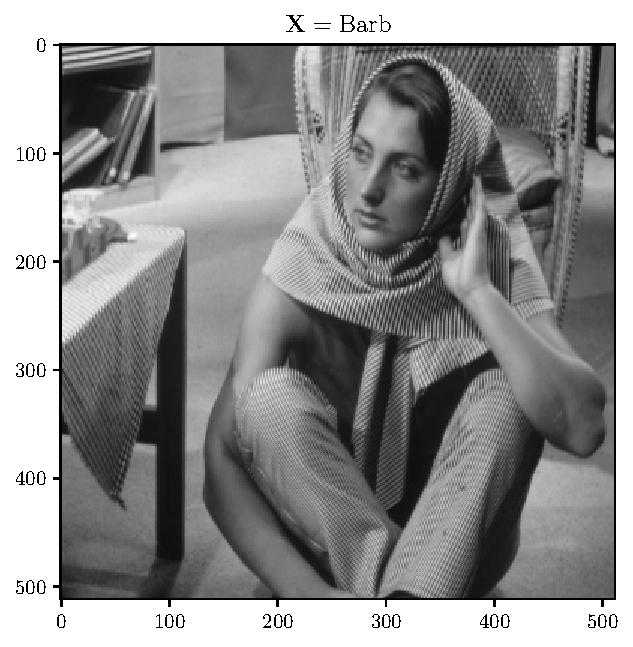
\includegraphics{barb.pdf}} & \href{https://nbviewer.org/github/vicente-gonzalez-ruiz/denoising/blob/main/notebooks/barb_0MMPG.ipynb\#barb_0MMPG}{\includegraphics{barb_0MMPG.pdf}} \\
      \href{https://nbviewer.org/github/vicente-gonzalez-ruiz/denoising/blob/main/notebooks/barb_averaging.ipynb\#barb_averaging}{\includegraphics{barb_averaging.pdf}} & \href{https://nbviewer.org/github/vicente-gonzalez-ruiz/denoising/blob/main/notebooks/barb_averaging_PSNR.ipynb\#barb_averaging_PSNR}{\includegraphics{barb_averaging_PSNR.pdf}}
    \end{tabular}
  }
  \caption{Increase of the SNR as a function of the number of noisy
    instances used in MNI. The clean image is shown on the top-left,
    and a noisy instance on the top-right. On to bottom-left, the
    denoised NMI image, and on the bottom-right the progression of the
    SNR as a function of $I$ and the level of
    noise.\label{fig:MNI_0MMPG}}
\end{figure}

\begin{comment}
%{{{

Fig.~\ref{fig:0MAUN} shows an
example of how zero-mean uniform noise is cancelled by averaging.
  
  \begin{figure}
    \centering
    \resizebox{1.0\textwidth}{!}{
      \renewcommand{\arraystretch}{0.0} % Adjust row spacing in the table
      \setlength{\tabcolsep}{0ex}      % Adjust column spacing in the table    
      \begin{tabular}{cc}
        \href{https://nbviewer.org/github/vicente-gonzalez-ruiz/denoising/blob/main/figs/averaging_denoising.ipynb\#Display-Barb}{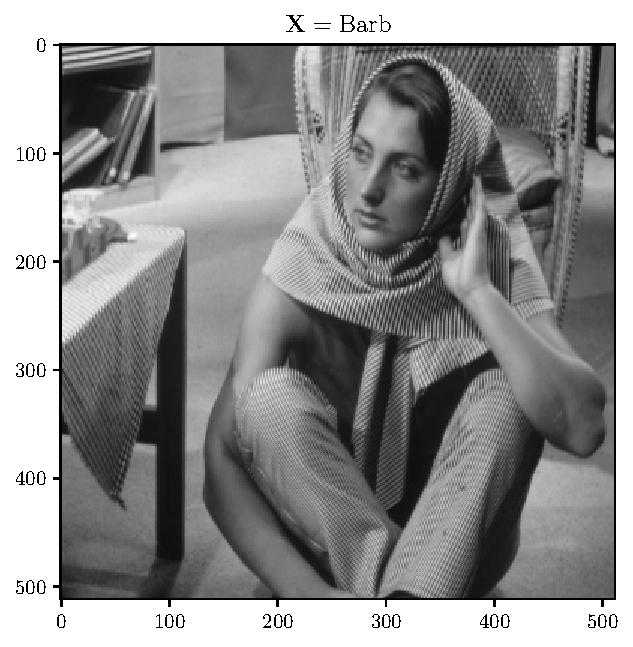
\includegraphics{barb}} & \href{https://nbviewer.org/github/vicente-gonzalez-ruiz/denoising/blob/main/figs/averaging_denoising.ipynb\#0MAUN_barb}{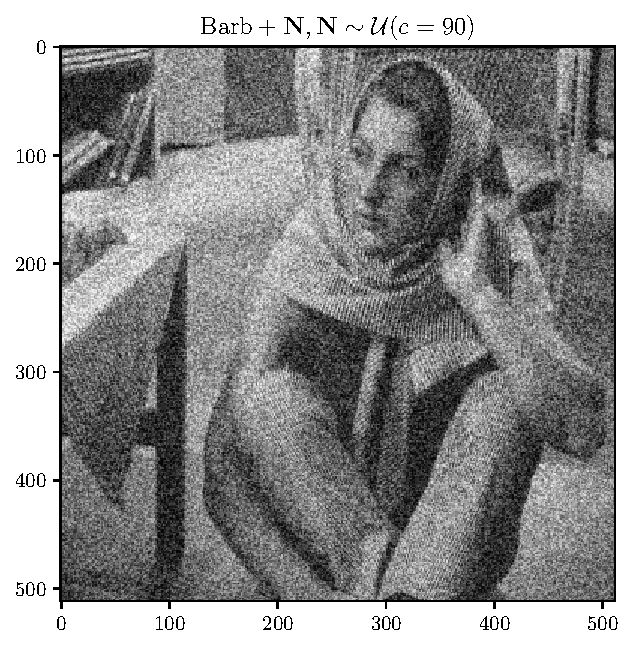
\includegraphics{0MAUN_barb}} \\
        \href{https://nbviewer.org/github/vicente-gonzalez-ruiz/denoising/blob/main/figs/averaging_denoising.ipynb\#denoised_0MAUN_barb}{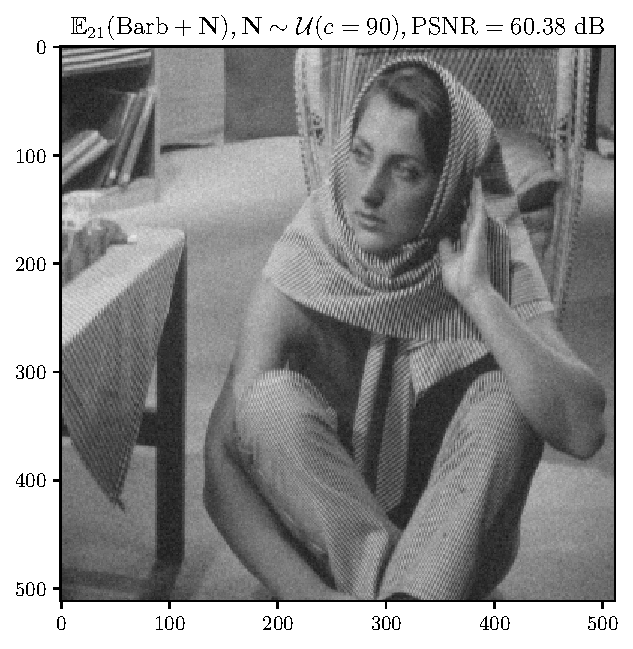
\includegraphics{denoised_0MAUN_barb}} & \href{https://nbviewer.org/github/vicente-gonzalez-ruiz/denoising/blob/main/figs/averaging_denoising.ipynb\#PSNR_0MAUN_barb}{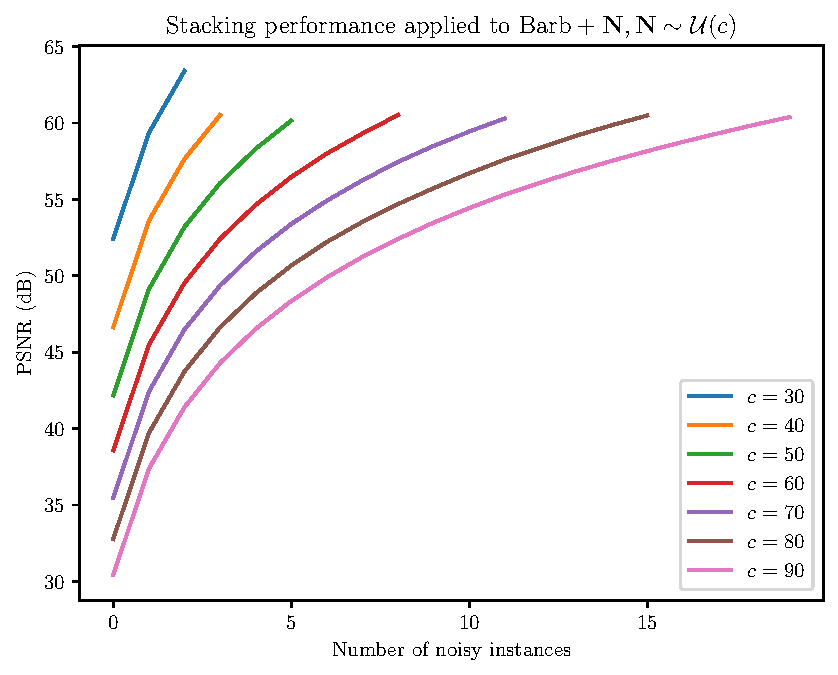
\includegraphics{PSNR_0MAUN_barb}}
      \end{tabular}
    }
    \caption{Effect of zero-mean additive uniform noise in an image
      and how averaging can be used to reduced by averaging. The clean
      image of Barb is shown on the top left, and a noisy version on
      the top right. On to bottom, the left image shows a denoised
      version after averaging and the right graph shows the performance
      of the averaging process for different levels of
      noise.\label{fig:0MAUN}}
  \end{figure}

 Fig.~\ref{fig:0MAGN} shows an
  example of how zero-mean Gaussian noise is cancelled by averaging.

  \begin{figure}
    \centering
    \resizebox{1.0\textwidth}{!}{
      \renewcommand{\arraystretch}{0.0} % Adjust row spacing in the table
      \setlength{\tabcolsep}{0ex}      % Adjust column spacing in the table    
      \begin{tabular}{cc}
        \href{https://nbviewer.org/github/vicente-gonzalez-ruiz/denoising/blob/main/figs/averaging_denoising.ipynb\#barb}{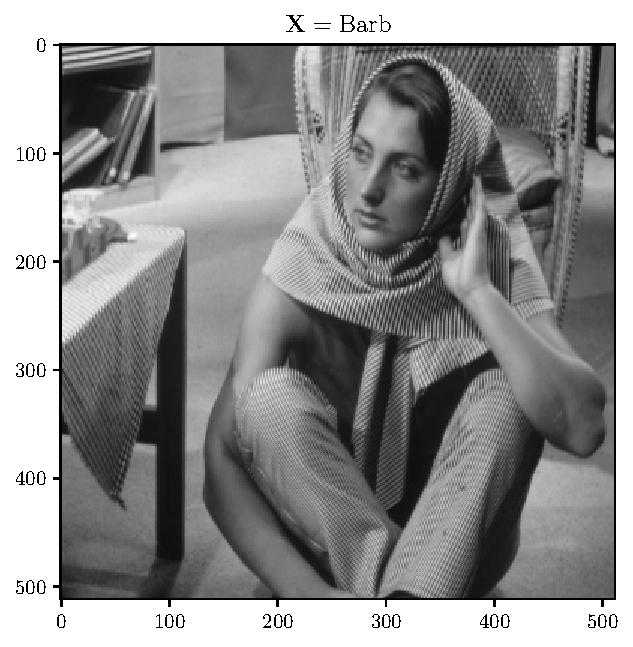
\includegraphics{barb}} & \href{https://nbviewer.org/github/vicente-gonzalez-ruiz/denoising/blob/main/figs/averaging_denoising.ipynb\#0MAGN_barb}{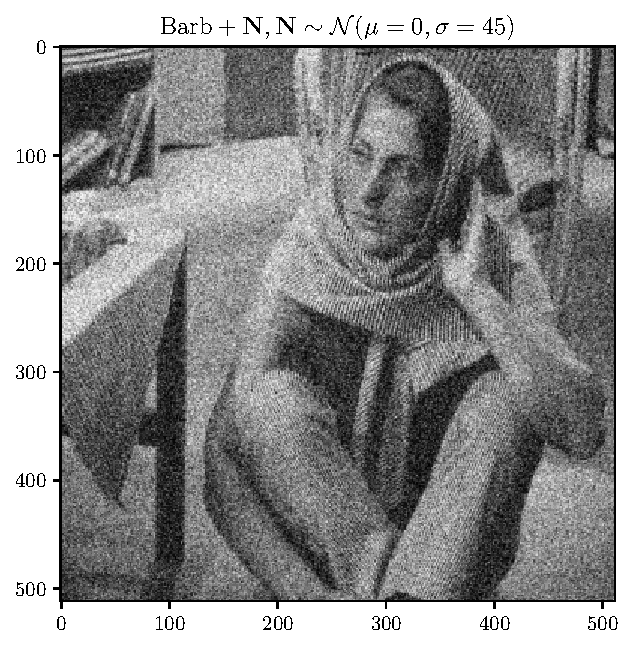
\includegraphics{0MAGN_barb}} \\
        \href{https://nbviewer.org/github/vicente-gonzalez-ruiz/denoising/blob/main/figs/averaging_denoising.ipynb\#denoised_0MAGN_barb}{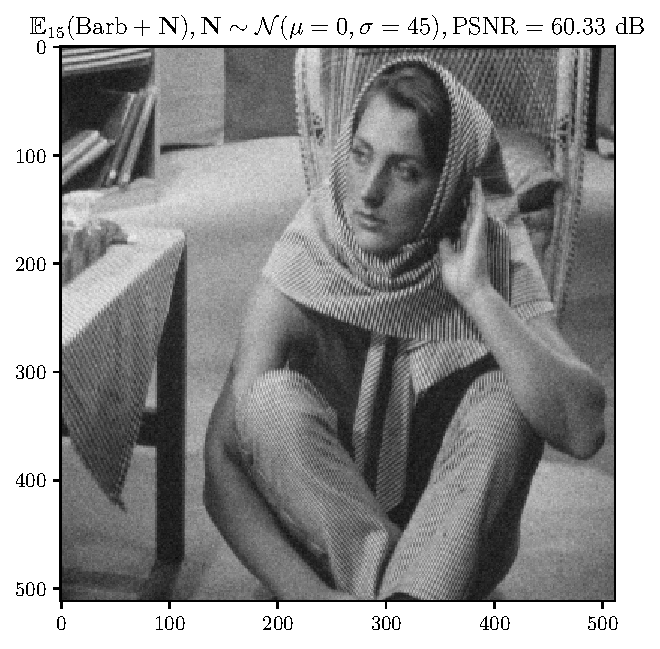
\includegraphics{denoised_0MAGN_barb}} & \href{https://nbviewer.org/github/vicente-gonzalez-ruiz/denoising/blob/main/figs/averaging_denoising.ipynb\#PSNR_0MAGN_barb}{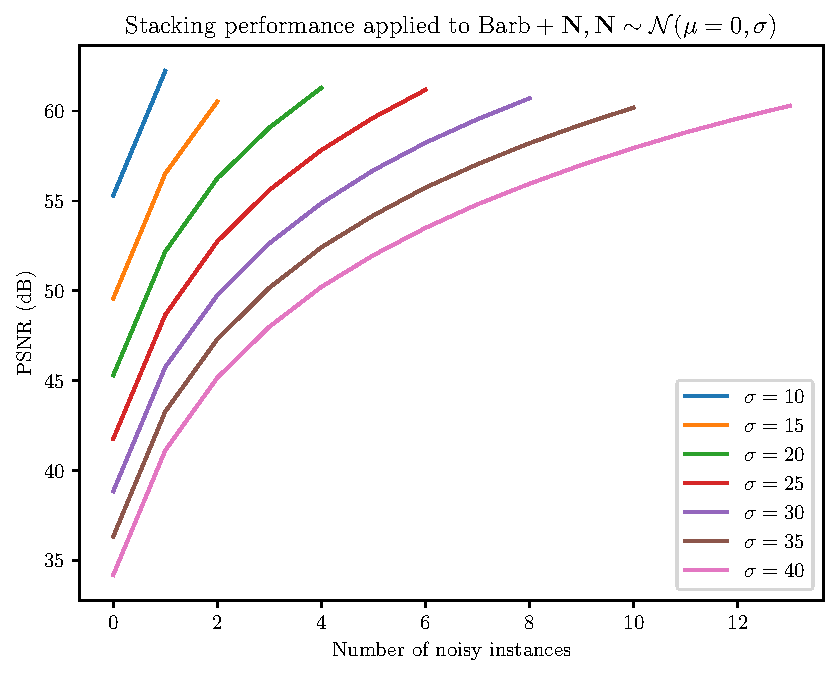
\includegraphics{PSNR_0MAGN_barb}}
      \end{tabular}
    }
    \caption{Effect of zero-mean additive Gaussian noise in an image
      and how averaging can be used to reduced by averaging. The clean
      image of Barb is shown on the top left, and a noisy version on
      the top right. On to bottom, the left image shows a denoised
      version after averaging and the right graph shows the performance
      of the averaging process for different levels of
      noise.\label{fig:0MAGN}}
  \end{figure}

  Fig.~\ref{fig:0MMGN} shows an example of
  how zero-mean Gaussian noise is cancelled by averaging.

  \begin{figure}
    \centering
    \resizebox{1.0\textwidth}{!}{
      \renewcommand{\arraystretch}{0.0} % Adjust row spacing in the table
      \setlength{\tabcolsep}{0ex}      % Adjust column spacing in the table    
      \begin{tabular}{cc}
        \href{https://nbviewer.org/github/vicente-gonzalez-ruiz/denoising/blob/main/figs/averaging_denoising.ipynb\#barb}{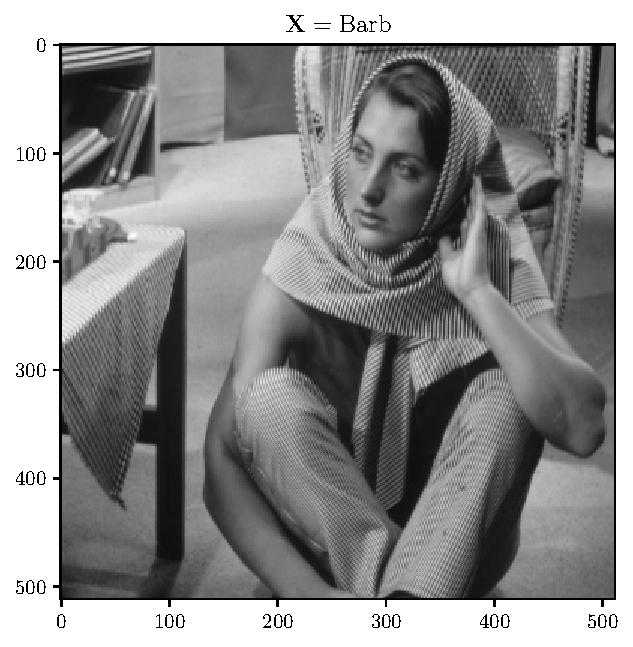
\includegraphics{barb}} & \href{https://nbviewer.org/github/vicente-gonzalez-ruiz/denoising/blob/main/figs/averaging_denoising.ipynb\#0MMGN_barb}{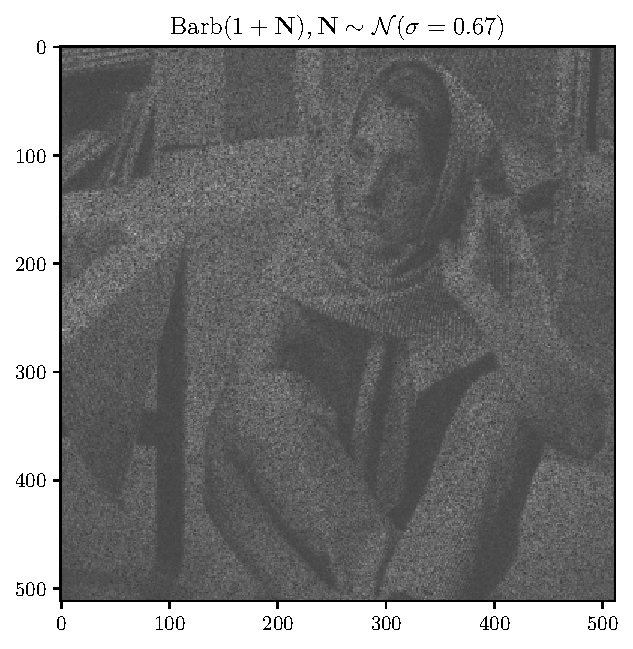
\includegraphics{0MMGN_barb}} \\
        \href{https://nbviewer.org/github/vicente-gonzalez-ruiz/denoising/blob/main/figs/averaging_denoising.ipynb\#denoised_0MMGN_barb}{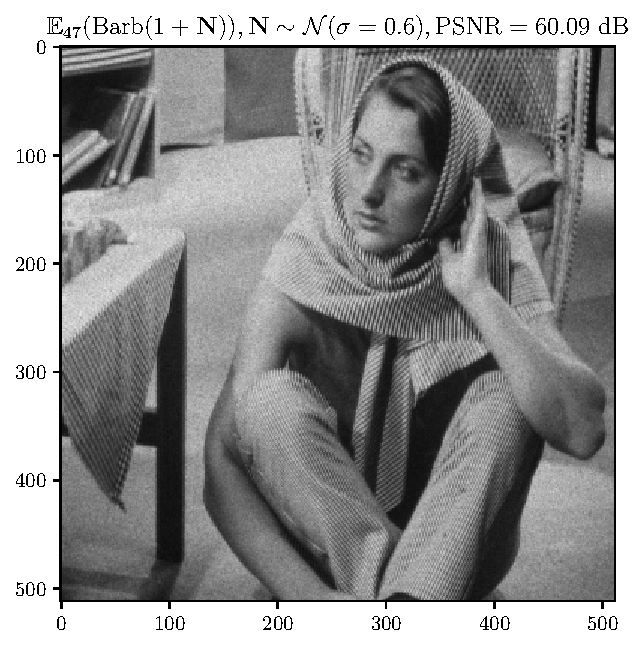
\includegraphics{denoised_0MMGN_barb}} & \href{https://nbviewer.org/github/vicente-gonzalez-ruiz/denoising/blob/main/figs/averaging_denoising.ipynb\#PSNR_0MMGN_barb}{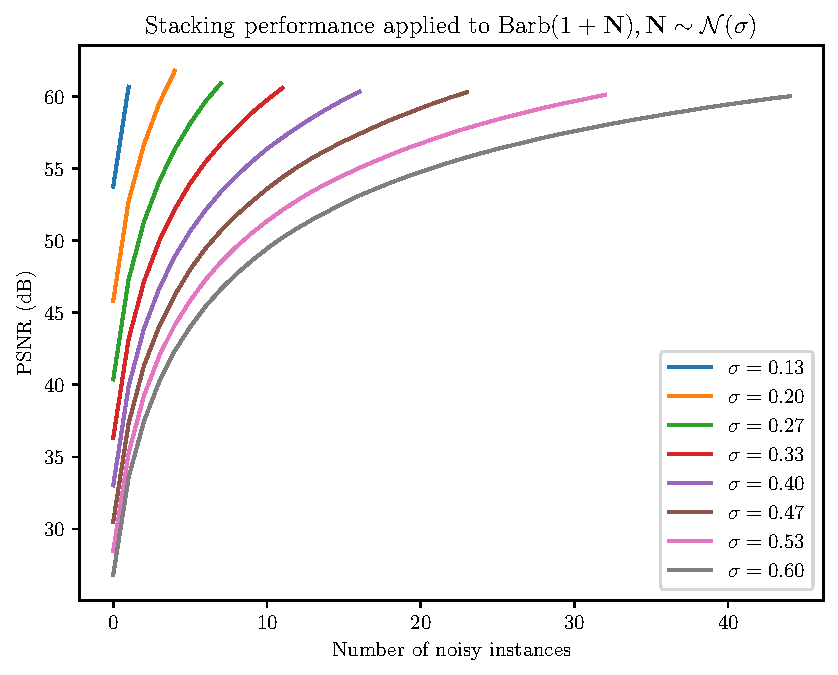
\includegraphics{PSNR_0MMGN_barb}}
      \end{tabular}
    }
    \caption{Effect of zero-mean multiplicative Gaussian noise in an
      image and how averaging can be used to reduced by averaging. The
      clean image of Barb is shown on the top left, and a noisy
      version on the top right. On to bottom, the left image shows a
      denoised version after averaging and the right graph shows the
      performance of the averaging process for different levels of
      noise.\label{fig:0MMGN}}
  \end{figure}

 Fig.~\ref{fig:Rayleigh}
  shows an example of how Rayleigh noise is cancelled by averaging.

  \begin{figure}
    \centering
    \resizebox{1.0\textwidth}{!}{
      \renewcommand{\arraystretch}{0.0} % Adjust row spacing in the table
      \setlength{\tabcolsep}{0ex}      % Adjust column spacing in the table    
      \begin{tabular}{cc}
        \href{https://nbviewer.org/github/vicente-gonzalez-ruiz/denoising/blob/main/figs/averaging_denoising.ipynb\#barb}{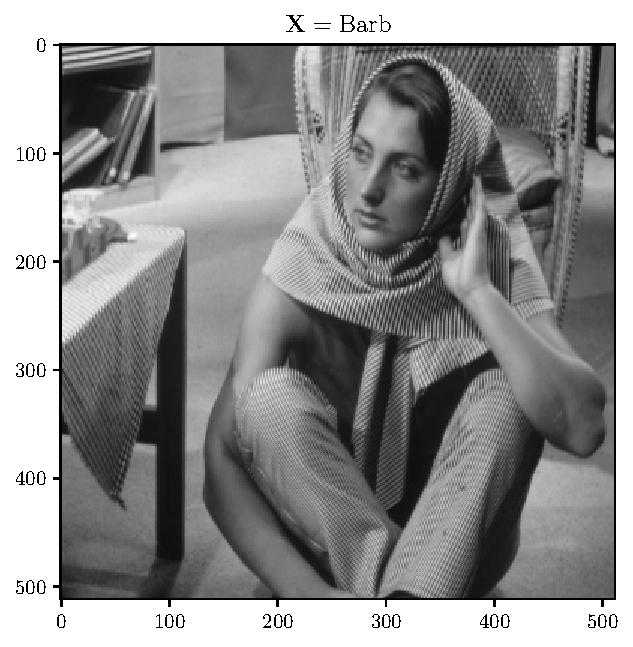
\includegraphics{barb}} & \href{https://nbviewer.org/github/vicente-gonzalez-ruiz/denoising/blob/main/figs/averaging_denoising.ipynb\#Rayleigh_barb}{\includegraphics{Rayleigh_barb}} \\
        \href{https://nbviewer.org/github/vicente-gonzalez-ruiz/denoising/blob/main/figs/averaging_denoising.ipynb\#denoised_Rayleigh_barb}{\includegraphics{denoised_Rayleigh_barb}} & \href{https://nbviewer.org/github/vicente-gonzalez-ruiz/denoising/blob/main/figs/averaging_denoising.ipynb\#PSNR_Rayleigh_barb}{\includegraphics{PSNR_Rayleigh_barb}}
      \end{tabular}
    }
    \caption{Effect of Rayleigh noise in an image and how averaging can
      be used to reduced by averaging. The clean image of Barb is shown
      on the top left, and a noisy version on the top right. On to
      bottom, the left image shows a denoised version after averaging
      and the right graph shows the performance of the averaging
      process for different levels of noise.\label{fig:Rayleigh}}
  \end{figure}

  Fig.~\ref{fig:Poisson} shows an example of how Poisson noise is
  cancelled by averaging.

  \begin{figure}
    \centering
    \resizebox{1.0\textwidth}{!}{
      \renewcommand{\arraystretch}{0.0} % Adjust row spacing in the table
      \setlength{\tabcolsep}{0ex}      % Adjust column spacing in the table    
      \begin{tabular}{cc}
        \href{https://nbviewer.org/github/vicente-gonzalez-ruiz/denoising/blob/main/figs/averaging_denoising.ipynb\#barb}{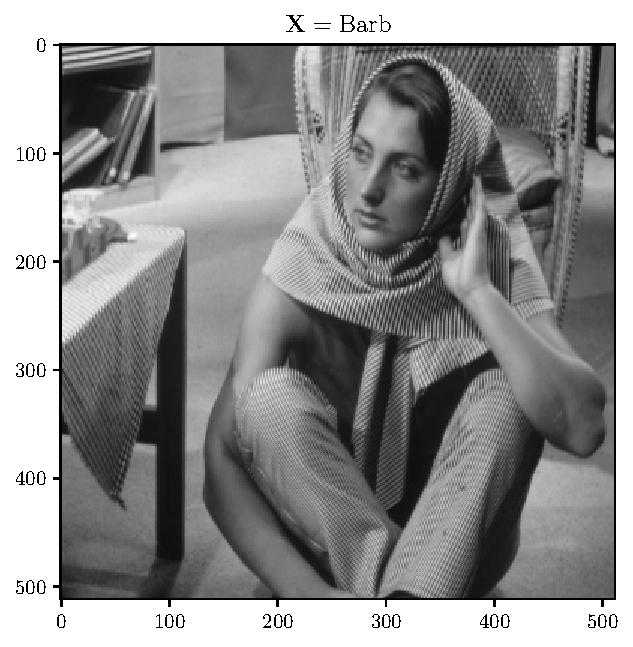
\includegraphics{barb}} & \href{https://nbviewer.org/github/vicente-gonzalez-ruiz/denoising/blob/main/figs/averaging_denoising.ipynb\#Poisson_barb}{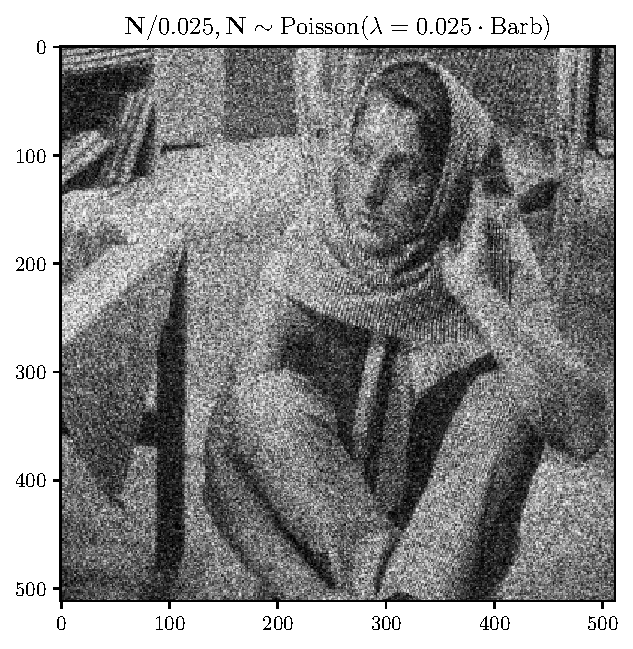
\includegraphics{Poisson_barb}} \\
        \href{https://nbviewer.org/github/vicente-gonzalez-ruiz/denoising/blob/main/figs/averaging_denoising.ipynb\#denoised_Poisson_barb}{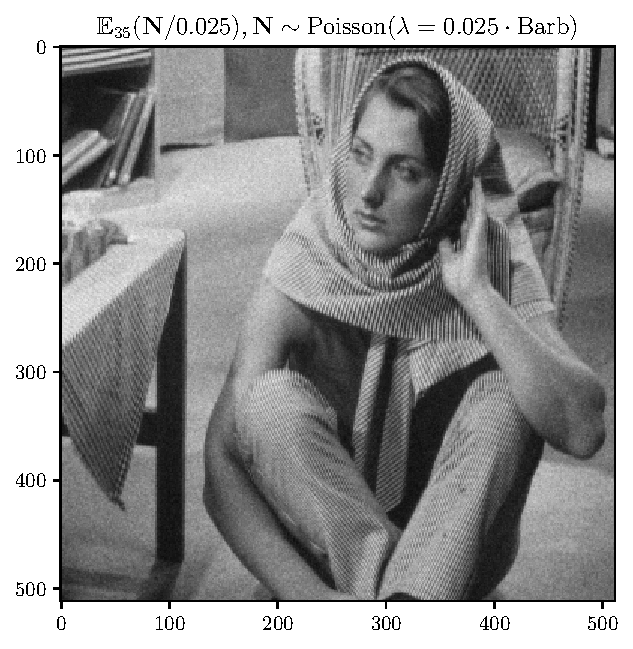
\includegraphics{denoised_Poisson_barb}} & \href{https://nbviewer.org/github/vicente-gonzalez-ruiz/denoising/blob/main/figs/averaging_denoising.ipynb\#PSNR_Poisson_barb}{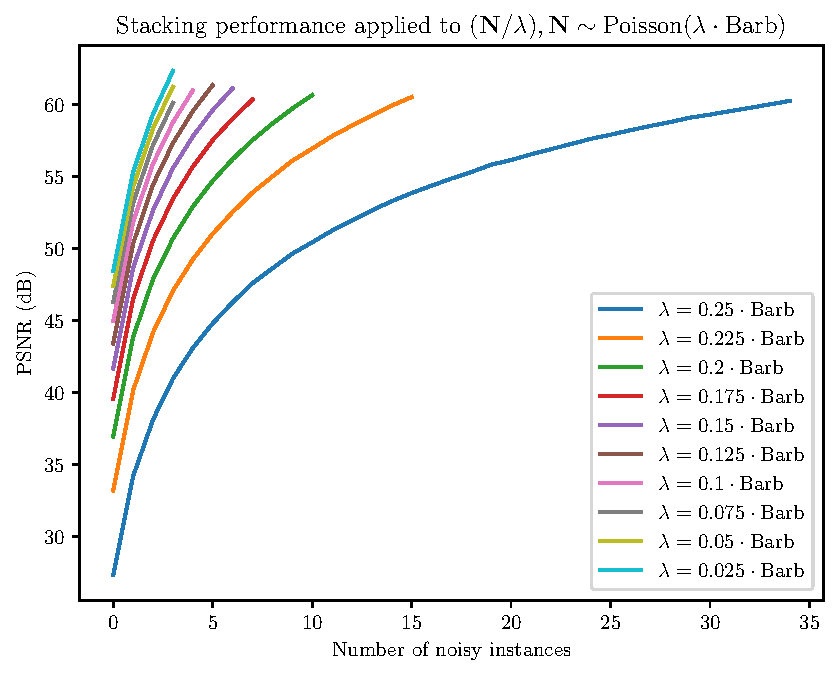
\includegraphics{PSNR_Poisson_barb}}
      \end{tabular}
    }
    \caption{Effect of Poisson noise in an image and how averaging can
      be used to reduced by averaging. The clean image is shown
      on the top left, and a noisy version on the top right. On the
      bottom, the left image shows a denoised version after averaging
      and the right graph shows the performance of the averaging
      process for different levels of noise.\label{fig:Poisson}}
  \end{figure}

%}}}
\end{comment}

%}}}

%\section{Beltrami flow}

%\section{Median filter}

%\section{Bilateral filter}

\subsection{Gaussian Filtering (GF)}
%{{{

In GF denoising, a 1D Gaussian kernel $h$ is convolved with the noisy
instance $\hat{\mathbf{X}}$ to obtain
\begin{equation}
  \tilde{\mathbf{X}} = \hat{\mathbf{X}}*\mathbf{h},
  \label{eq:GF}
\end{equation}
where $\tilde{\mathbf{X}}$ represents the denoised signal, and $*$ the
convolution of digital signals. As can be seen, unlike MNI, GF only
requires a noisy instance.

The coefficients of $h$ define a low-pass\footnote{We can distinguish
  this because all are positive coefficients.} filter. They are
sampled from
\begin{equation}
  \mathbf{h}(x) = \frac{1}{\sqrt{2\pi}\tau}e^{-\frac{{x}^2}{(2\tau^2)}},
  \label{eq:GK}
\end{equation}
where $x$ represents a distance in
the signal domain, and $\tau$ (known as the \emph{standard deviation}
\footnote{Notice that the filter coefficients are also the values that a
  discrete random variable takes from a normal distribution.})
determines the bandwidth of the filter.

\begin{figure}
  \centering
  \includegraphics[width=0.8\textwidth]{3D_GF}
  \caption{3D Gaussian filtering. The gray planes contain the voxels
    that are filtered and the white planes contain the voxels used by
    the 1D kernel when it is applied to the voxels of the filtered
    plane. The kernel shown here contains 3 coefficients. The volume
    is convolved sequentially in-place, from left to
    right.\label{fig:3D_GF}}
\end{figure}

Multidimensional GF is separable (see
Appendix~\ref{ape:GF_separability}), which means that we
can apply the 1D filter to the $D$ dimensions of the signal to compute
a $D$D denoising. For the 3D case (see Fig.~\ref{fig:3D_GF}), we have
that
\begin{equation}
  \tilde{\mathbf{X}} = \Big(\big(\hat{\mathbf X}*^{(\text{Z})}{\mathbf h}\big)*^{(\text{Y})}{\mathbf h}\Big)*^{(\text{X})}{\mathbf h},
    \label{eq:3D_GF}
\end{equation}
where ${\mathbf s}*^{(d)}{\mathbf h}$ is the 1D convolution applied to
the dimension $d$ of the signal ${\mathbf s}$ and the (1D) filter
${\mathbf h}$. For simplicity, Eq.~\ref{eq:3D_GF} defines isotropic
filtering, but $\tau$ can be different at each dimension to provide
anisotropy.

\begin{figure}
  \centering
  \resizebox{1.0\textwidth}{!}{
    \renewcommand{\arraystretch}{0.0} % Adjust row spacing in the table
    \setlength{\tabcolsep}{0ex}      % Adjust column spacing in the table    
    \begin{tabular}{cc}
      \href{https://nbviewer.org/github/vicente-gonzalez-ruiz/denoising/blob/main/notebooks/barb_GF_optimal_tau.ipynb\#barb_GF_optimal_tau}{\includegraphics{barb_GF_optimal_tau.pdf}} & \href{https://nbviewer.org/github/vicente-gonzalez-ruiz/denoising/blob/main/notebooks/lake_GF_optimal_tau.ipynb\#lake_GF_optimal_tau}{\includegraphics{lake_GF_optimal_tau.pdf}}
    \end{tabular}
  }
  \caption{Optimal $\tau$ values in GF. {\color{red} Ojo, son iguales}\label{fig:optimal_GF_tau}}
\end{figure}

As can be seen in Eqs.~\ref{eq:1D_GF} and \ref{eq:3D_GF}, the
denoising result depends on $\tau$. An optimal value for $\tau$
($\tau^*$) can be found if we know $\mathbf{X}$ (see
Fig.~\ref{fig:optimal_GF_tau}). Unfortunately, $\mathbf{X}$ is usually
unknown and we only can estimate $\tau^*$. Ideally, $\tau^*$ should
increase the SNR as much as possible, considering also that: (1) GF
attenuates the high frequencies, (2) the SFC of the noise is close to
zero, and (3) that most of the energy (information) in the signals are
concentrated in the low frequencies. Therefore, we should find a cut-off frequency
\begin{equation}
  \eta^* = \text{min}\{\eta|\text{SFC}(\hat{\mathbf{X}})_\eta < \beta\}
\end{equation}
that attenuates those high frequency components of
$\hat{\mathbf{X}}$ where the SFC is smaller than a given threshold
$\beta$.

In the Appendix~\ref{ape:tau_VS_beta} it is shown how to find
$\tau^*$, in the continuous case, known the cut-off frequency $\eta$
and $\beta$. Concretelly, the relation between these variables is
\begin{equation}
  \tau^* = \frac{\sqrt{-2\ln\beta}}{\eta^*}.
  \label{eq:tau_VS_beta_eta}
\end{equation}

(habría que ver lo que ha dicho ChatGPT sobre el caso discreto
)
Unfortunately, for the discrete case, where we are working with
normalized frequencies and the $\text{size}(h)$ is finite (see
Appendix~\ref{ape:creation_GK}), Eq.~\ref{eq:tau_VS_beta_eta} is not
exact because $\text{size}(h)$ has also an impact in how $\tau^*$
should be found. As shown in Appendix~\ref{ape:creation_GK},
$\text{size}(h)$ depends on the implementation

\begin{comment}
%{{{

Assuming that most of the signal energy (information) is concentrated
in the low frequencies, higher values of $\tau$ will produce a higher
smoothing effect in $\tilde{\mathbf{X}}$). More concretely, if
$\mathcal{F}(h)=H$, that is
\begin{equation}
  H(u) = e^{-\frac{u^2}{2\tau^{-2}}},
\end{equation}
it can be seen that if $\tau$ increases, the cut-off frequency
provided by $H$ decreases, and viceversa. 


\begin{figure}
  \centering
  \resizebox{1.0\textwidth}{!}{
    \renewcommand{\arraystretch}{0.0} % Adjust row spacing in the table
    \setlength{\tabcolsep}{0ex}      % Adjust column spacing in the table    
    \begin{tabular}{cc}
      \href{https://nbviewer.org/github/vicente-gonzalez-ruiz/denoising/blob/main/notebooks/barb.ipynb}{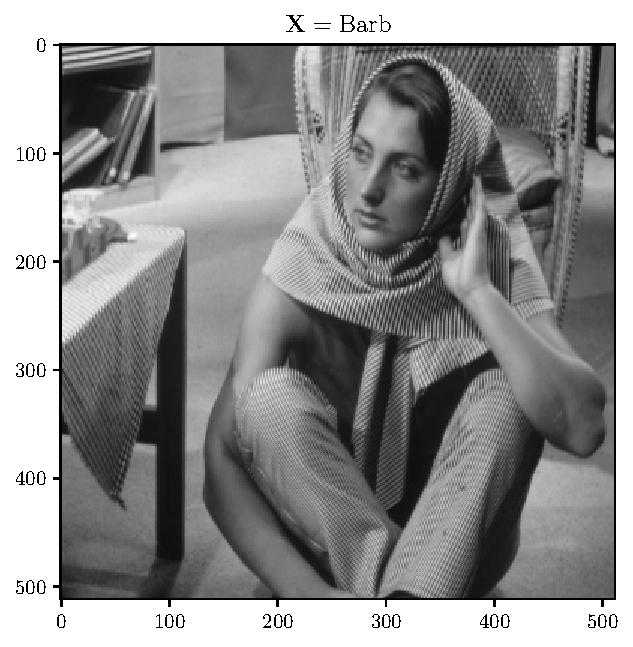
\includegraphics{barb}} & \href{https://nbviewer.org/github/vicente-gonzalez-ruiz/denoising/blob/main/figs/lake.ipynb}{\includegraphics{lake}} \\
      \href{https://nbviewer.org/github/vicente-gonzalez-ruiz/denoising/blob/main/notebooks/tau_VS_img.ipynb\#0MMPG_barb}{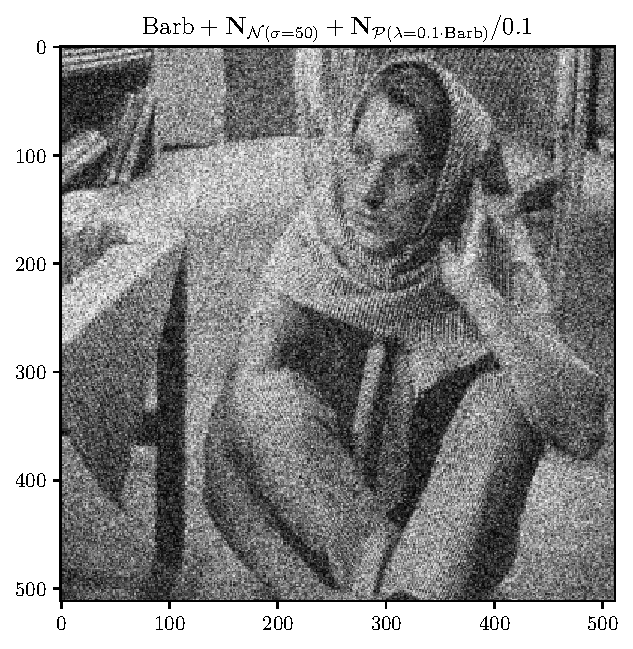
\includegraphics{0MMPG_barb}} & \href{https://nbviewer.org/github/vicente-gonzalez-ruiz/denoising/blob/main/figs/tau_VS_img.ipynb\#0MMPG_lake}{\includegraphics{0MMPG_lake}} \\
      \href{https://nbviewer.org/github/vicente-gonzalez-ruiz/denoising/blob/main/notebooks/tau_VS_img.ipynb\#GF_0MMPG_barb}{\includegraphics{GF_0MMPG_barb}} & \href{https://nbviewer.org/github/vicente-gonzalez-ruiz/denoising/blob/main/figs/tau_VS_img.ipynb\#GF_0MMPG_lake}{\includegraphics{GF_0MMPG_lake}}
    \end{tabular}
  }
  \caption{Two examples of optimal denoising using GF. On the top, the
    original images. In the middle, the noisy instances. On the
    bottom, the denoised images. {\color{red} arreglar PSNRs y elegir
      tau optimo para ejemplo}\label{fig:GF_tau_optimal}}
\end{figure}

Fig.~\ref{fig:tau_VS_image} shows the denoising performance of GF for
two artificially noised images, for different levels of noise
($\sigma$) and filter length ($\tau$). As can be seen, the optimal
value of the filter length, $\tau^*$ (which maximizes the PCC between
$\mathbf{X}$ and $\tilde{\mathbf{X}}$), depends on the noise level and
$\mathbf{X}$, information that is, in general, unavailable in
microscopy imaging. Therefore, $\tau^*$ can be only
\emph{estimated}\footnote{Notice that, only knowing $\mathbf{X}$ it
  would be possible to find $\tau^*$. Therefore, the furthest one can
  go is to estimate the optimal filtering parameters}. depending on,
for example, the (subjective) visual quality of
$\tilde{\mathbf{X}}$. An example of optimal denoising using GF has
been show in Fig.~\ref{fig:GF_tau_optimal}.

% \begin{figure}
%   \centering
%   \resizebox{1.0\textwidth}{!}{
%     \renewcommand{\arraystretch}{0.0} % Adjust row spacing in the table
%     \setlength{\tabcolsep}{0ex}      % Adjust column spacing in the table    
%     \begin{tabular}{cc}
%   \href{https://nbviewer.org/github/vicente-gonzalez-ruiz/denoising/blob/main/figs/gaussian_denoising.ipynb\#GD_SFRC_0MMPG_NL20_barb}{\includegraphics{GD_SFRC_0MMPG_NL20_barb}} & \href{https://nbviewer.org/github/vicente-gonzalez-ruiz/denoising/blob/main/figs/gaussian_denoising.ipynb\#GD_SFRC_0MMPG_NL60_barb}{\includegraphics{GD_SFRC_0MMPG_NL60_barb}}
%     \end{tabular}
%     }
%     \caption{SFRC curves for two different noisy instances of
%       Barb, see Fig.~\ref{fig:tau_VS_image} using two
%       different noise levels ($\sigma=20$ and $\sigma=60$), and after
%       having applied GD for several filter lengths. As can be seen, for $\sigma=20$, the ``optimal'' filter
%       length (that maximizes the area below the curve) is ..., and for
%       $\sigma=60$, the ``optimal'' filter length is ... Therefore, the
%       ``optimal'' filter length is (positively) correlated with the
%       noise level. Notice that $\tau$
%       has been discretized in steps of $0.25$.

%       (2) the
%       ``optimal'' filter length is (positively) correlated with the
%       noise level (for the noise level $\sigma=40$ and $\gamma=0.15$
%       the ``optimal'' $\tau=1.0$ and the noise level $\sigma=50$ and
%       $\gamma=0.15$ the ``optimal'' $\tau=1.25$). Notice that $\tau$
%       has been discretized in steps of $0.25$.


%       Relation between the SFRC curves and the filter length of
%       a Gaussian filter. $\hat{\mathbf{X}}_1$ is the the noise image
%       (Barb) shown in the Fig.~\ref{fig:tau_VS_image} (for $\sigma=40$
%       and $\gamma=0.15$). As can be seen, the area below the curve is
%       maximized for $\tau=1.0$

%       Effect of zero-mean MPG noise in an image and how GD
%     can be used to reduce it. A noisy version of the
%     image is on the top-left. On the top-right, the SFRC curves
%     of the denoised image for different filter lengths. As can be seen
%     in this subfigure, for the noise level
%     $(\sigma=40, \gamma=0.15)$, an optimal $\tau=1.25$ should be used if
%     (considering that the area below the SFRC curve should be maximized).
%     On the bottom-left, it can be seen that for this noise level,
%     the ``optimal'' Gaussian kernel-lenght is $\tau/2=0.625 \approx 0.7$. The resulting
%     ``optimal'' filtered image (using GD) is shown on the bottom-right.
%     \label{fig:GD_0MMPG}}
% \end{figure}

{\color{red} ------ comienzo sin terminar ------ }

It is also possible to estimate $\tau^*$ using the self-correlation in
the Fourier domain \cite{koho2019fourier} {\color{red}Este sería un
  buen punto para hablar de cómo estamos calculando la curva
  SF{R|S}C}. The idea here is to determine the frequency $u^*$ for
which, to the right of this frequency, the SNR decays under some given
threshold.

A more objective procedure to estimate $\tau^*$ should be based on
some (objective) quality metric, such as the self-correlation in the
Fourier domain \cite{koho2019fourier}. Fig.~\ref{fig:GD_0MMPG} shows
the result of using the SFRC of the noisy image to estimate $\tau^*$,
considering the idea that the low-pass filter should remove those
frequency components where the SNR is lower than a given threshold.



Fig.~\ref{fig:GD_0MMPG} shows
SFRC curves for different filter lengths, and it has been also
computed the normalized area below each curve, a metric that is
(positively) correlated with $\tau^*$ (see
Fig.~\ref{fig:tau_VS_image}). As can be seen that, $\tau^*$ can be
estimated using the filter length that maximizes the area below the
corresponding SFRC curve.


because the
higher the area, the higher also the PCC between the Fourier
coefficients


and it can be seen, the normalized area below the curve can be used to estimate


Another alternative can use some heuristic to estimate

We propose a more automatic procedure to find $\tau^*$.
by maximizing the ratio between the amount of noise and the amount of
signal removed by the filter. To determine this, we can use the SFRC
curve (see Sec.~\ref{sec:FSC}), in which each point represents the
correlation between two\footnote{Actually, each point is the average
  of two correlation coefficients, each one obtained after subsampling
  the image in each dimension (by rows, and by columns).} rings of
Fourier coefficients, extracted from two subsampled versions of
$\tilde{\mathbf{X}}$.

for the single parameter that GD requires (the length of
the Gaussian kernels in each dimension, represented by $\tau$ in
$\mathrm{GD}_\tau$) depends on the noise level, an information that is
generally unknown in microscopy imaging.

To estimate the relation between the filter length that should
maximize the quality of the denoised signal, the SFRC (Self Fourier
Ring Correlation, see Section~\ref{sec:FSC}) of several noisy
instances of the same image (variying the level of noise) has been
shown in the Fig.~\ref{fig:SFRC}.

has been calculated by subbands of a filtered
image, generating a number of SFRC curves, one for each different
kernel length $\tau$ (see Fig.  \ref{fig:GD_0MMPG}). As can be seen,
the autocorrelation increases when the noise level decreases due to
increasing $\tau$, until it reaches a value for which the
autocorrelation decreases again\footnote{Remember that the SFRC metric
  quantifies the correlation between subsampled versions of the same
  input signal and that, by definition, the MPG noise should be
  uncorrelated. For this reason, if noise were only had at the input,
  we should obtain a flat SFRC that approximates to zero. Therefore,
  the higher the area below the SFRC curve, the higher the presence of
  signal.}. For that $\tau^*$, which maximizes the area under the
curve up to the normalized frequency $\omega/4$, is when the PCC
metric is also maximized (considering the original image resolution,
i.e., without the subsampling required to compute the SFRC) for
$\tau^*/2$, which means that we can use the SFRC metric (in the 2D
case) and the SFSC (in the 3D case) to estimate the optimal filtering
parameters knowing only the noisy instance $\hat{\mathbf{X}}$.

{\color{red} ------ fin sin terminar ------ }

%}}}
\end{comment}


%}}}


% \section{Anisotropic Non-linear Diffusion (AND)}


\subsection{Structure-Preserving Gaussian Denoising (SPGD)}
%{{{

\begin{figure}
  \centering
  \includegraphics[width=\textwidth]{yes_OF_images}
  \caption{SPGD along the $\mathrm{Z}$-dimension. Five consecutive
    slices (or $\mathrm{XY}$-planes) are involved in the filtering of
    the slice $\hat{\mathbf{X}}_z$. Four displacements fields
    (represented by arrows) determined by the OF estimator are used
    for the alignment of the structures found in the slices
    $\hat{\mathbf{X}}_{z-2}, \hat{\mathbf{X}}_{z-1},
    \hat{\mathbf{X}}_{z+1},$ and $\hat{\mathbf{X}}_{z+2}$ with respect
    to those present in $\hat{\mathbf{X}}_{z-2}$, hence producing
    OF-compensated slices. The Gaussian filtering along the
    $\text{Z}$-dimension (dotted line) is then applied to the
    OF-compensated slices.\label{fig:SPGD}}
\end{figure}


SPGD is based in 3D Gaussian filtering (see Eq.~\ref{eq:3D_GD}), but
the noised volume $\hat{\mathbf{X}}$ is slice-wise 2D-warped (see
Fig. \ref{fig:SPGD}), in the 3 space dimensions (see
Fig. \ref{fig:3D_GD}), resulting (compared to GD) in a reduction of
the bluring of the structures detected by a 2D OF (Optical Flow)
estimator \cite{gonzalez2023structure}. This idea can be expressed as
\begin{equation}
  \tilde{\mathbf{X}}  = R_\text{X}\Big(R_\text{Y}\big(R_\text{Z}(\hat{\mathbf{X}})*^{(\text{Z})}{\mathbf h}\big)*^{(\text{Y})}{\mathbf h}\Big)*^{(\text{X})}{\mathbf h},
    \label{eq:SDPG}
\end{equation}
where
\begin{equation*}
    \begin{array}{rclll}
    R_\text{Z}(\hat{\mathbf{X}}) & = & \big\{ \{ \overset{z'\rightarrow z}p(\hat{\mathbf X}_{[z',:,:]})~:~\overset{z'\rightarrow z}p(\hat{\mathbf X}_{[z',:,:]})\approx\hat{\mathbf X}_{[z,:,:]} & \\ & & \text{for}
 ~z'=z-k,\cdots,z+k\} ~\text{for}~z=0,1,\cdots,N_\text{Z}-1\big\}, \\
    R_\text{Y}(\hat{\mathbf{X}}) & = & \big\{ \{ \overset{y'\rightarrow y}p(\hat{\mathbf X}_{[:,y',:]})~:~\overset{y'\rightarrow y}p(\hat{\mathbf X}_{[:,y',:]}\approx\hat{\mathbf X}_{[:,y,:]} & \\ & & \text{for}
 ~y'=y-k,\cdots,y+k\} ~\text{for}~y=0,1,\cdots,N_\text{Y}-1\big\},~\text{and} \\
    R_\text{X}(\hat{\mathbf{X}}) & = & \big\{ \{ \overset{x'\rightarrow x}p(\hat{\mathbf X}_{[:,:,x']})~:~\overset{x'\rightarrow x}p(\hat{\mathbf X}_{[:,:,x']}\approx\hat{\mathbf X}_{[:,:,x]} & \\ & & \text{for}
 ~x'=x-k,\cdots,x+k\} ~\text{for}~x=0,1,\cdots,N_\text{X}-1\big\}
    \end{array}
\end{equation*}
are the slice-wise warped volumes. For example,
$\overset{x'\rightarrow x}p(\hat{\mathbf X}_{[:,:,x']})$ represents
the projection of the slice at coordinate $x'$ fulfilling that
$\overset{x'\rightarrow x}p({\hat{\mathbf X}})\approx{\hat{\mathbf
    X}}_{[:,:,x]}$. Notice that, for each possible offset in
$\text{Z}$, $\text{Y}$, and $\text{X}$, a different set of
warped 2D slices must be computed.

Compared with GD denoising, the OF estimator requires some new
parameters \cite{farneback2003two}, but only the window size $w$, has
a high impact on the performance of the filtering process. If $w$ is
large, the estimator is less sensitive to the noise but also the small
structures are ignored. Therefore, higher $w$ values increases
blurring, and viceversa.

\begin{figure}
  \centering
  \resizebox{1.0\textwidth}{!}{
    \renewcommand{\arraystretch}{0.0} % Adjust row spacing in the table
    \setlength{\tabcolsep}{0ex}      % Adjust column spacing in the table    
    \begin{tabular}{cc}
      \href{https://nbviewer.org/github/vicente-gonzalez-ruiz/denoising/blob/main/figs/gaussian_denoising.ipynb\#GF_0MMPG_barb}{\includegraphics{GF_0MMPG_barb}} & \href{https://nbviewer.org/github/vicente-gonzalez-ruiz/denoising/blob/main/figs/OF_gaussian_denoising.ipynb\#SPGD_0MMPG_barb}{\includegraphics{SPGD_0MMPG_barb}} \\
      \href{https://nbviewer.org/github/vicente-gonzalez-ruiz/denoising/blob/main/figs/OF_gaussian_denoising.ipynb\#SPGD_SFRC_0MMPG_barb}{\includegraphics{SPGD_SFRC_0MMPG_barb}} & \href{https://nbviewer.org/github/vicente-gonzalez-ruiz/denoising/blob/main/figs/OF_gaussian_denoising.ipynb\#SPGD_PCC_0MMPG_barb}{\includegraphics{SPGD_PCC_0MMPG_barb}}
    \end{tabular}
  }
  \caption{Effect of zero-mean MPG noise in an image and how SPGD)
    can be used to reduce it. On the top-left, the best
    denoised version generated by GD. On the top-right, the best denoised version using
    SPGD. On the bottom-left it is shown the performance
    of SPGD for different levels of noise. On the bottom-right, the SFRC curves
    of the denoised image for different filter lengths. As can be seen
    in the bottom-left subfigure, for the noise level $(\sigma=30,
    \gamma=0.15)$, the optimal $\tau^*=7.0$. In the bottom-right
    subfigure it can be seen that for this noise level, the optimal
    Gaussian kernel-lenght is $\tau^*/2=3.5$.
    \label{fig:SPGD_0MMPG}}
\end{figure}

A set of experiments have been conducted to figure out:
\begin{enumerate}
\item The relationship between $\tau$, $l$, and $w$.
\item Whether the self correlation in the Fourier domain of the
  denoised image can estimate optimal values for these parameters.
\end{enumerate}

Fig.~\ref{fig:SPGD_0MMPG} shows the performance of SPGD in a artificially
noised image, for different levels of noise. As can be seen, the
optimal value for the single parameter that SPGD requires (the length of
the Gaussian kernels in each dimension) depends on the noise level, an
information that is generally unknown in microscopy imaging.

%}}}

%\subsection{Non Local Means (NLM)} 

%\subsection{BM4D}



% \section{N2V}
% A. Krull, T.-O. Buchholz, and F. Jug, “Noise2void-learning denoising
% from single noisy images,” in Proceedings of the IEEE/CVF conference
% on computer vision and pattern recognition, 2019, pp. 2129–2137.

\subsection{Cryo-CARE}
%{{{

CARE (Content-Aware image REstoration) methods leverage available
knowledge about the data at hand ought to yield superior restoration
results \cite{weigert2018content}. Concretely, Cryo-CARE
\cite{buchholz2019cryo} is an implementation of Noise2Noise (N2N)
\cite{lehtinen2018noise2noise}.

N2N is a ``supervised'' learning method for denoising where an
autoencoder neural network with skip connections (a U-Net) is trained
on pairs of noisy images. However, unlike clasical supervised
denoising deep-learning based models, that usually implement
\cite{lehtinen2018noise2noise}
\begin{equation}
  \underset{\theta}{\operatorname{arg\,min}} \, \sum_j L \big(f_\theta(\hat{\mathbf X}_j^{(1)}), {\mathbf X}_j\big)
\end{equation}
\begin{equation}
  \underset{\theta}{\operatorname{arg\,min}} \, \sum_j L \big(f_\theta(\{\hat{\mathbf X}\}_j), \{{\mathbf X}\}_j\big)
\end{equation}

where $\{(\hat{\mathbf{X}}, \mathbf{X})\}_j\}$ is the training
dataset, and $L$ is a given lost function such as the MSE, N2N solve

where $\{(\hat{\mathbf X}_j^{(1)}, {\mathbf X}_j)\}_{j=1}^M$ is the training
dataset, and $L$ is a given lost function such as the MSE, N2N solves
\begin{equation}
  \underset{\theta}{\operatorname{arg\,min}} \, \sum_j L \big(f_\theta(\hat{\mathbf X}_j^{(1)}), {\mathbf X}_j^{(2)}\big).
\end{equation}
In other words, given two noisy versions
$\{\hat{\mathbf Y}^{(1)}, \hat{\mathbf Y}^{(2)}\}$ of the same (clean)
volume ${\mathbf Y}$, N2N learns to infeer a denoised volume
\begin{equation}
  \tilde{\mathbf Y}=\frac{1}{2}\big(f_\theta(\hat{\mathbf Y}^{(1)})+f_\theta(\hat{\mathbf Y}^{(2)})\big)\approx{\mathbf Y}.
\end{equation}
Obviously, better approximations to ${\mathbf Y}$ will be obtained
having more noisy instances, after averaing all the denoised volumes.

%}}}

\subsection{2D Random Shuffing Volume Denoising (2D-RSVD)}

\subsection{3D Random Shuffling Volume Denoising (3D-RSVD)}

%}}}

\appendix

\section{Fourier transform of a Gaussian function}
%{{{

The Fourier transform of a continuous Gaussian function
\begin{equation*}
  h(x) = \frac{1}{\sqrt{2\pi}\tau}e^{-\frac{{x}^2}{(2\tau^2)}},
\end{equation*}
(see Eq.~\ref{eq:GF}) is
\begin{equation}
  H(w) = \mathcal{F}\{h(x)\} = \int_{-\infty}^{\infty}h(x)e^{-jwx}dx,
\end{equation}
where
\begin{equation}
  w = 2\pi f,
\end{equation}
representing $f$ frequency (in the case of working with images, in
cycles per pixel size measured in units of distance, or simply, cycles
per sample) and $w$ angular frequency (radians per unit distance, or
simply, radians per sample). Therefore,
\begin{equation*}
  H(w) = \int_{-\infty}^{\infty}\frac{1}{\sqrt{2\pi}\tau}e^{-\frac{x^2}{2\tau^2}}e^{-jwx}dx = 
\end{equation*}
\begin{equation*}
  \frac{1}{\sqrt{2\pi}\tau}\int_{-\infty}^{\infty}e^{-\frac{x^2}{2\tau^2}}e^{-jwx}dx = 
\end{equation*}
\begin{equation*}
  \frac{1}{\sqrt{2\pi}\tau}\int_{-\infty}^{\infty}e^{-\frac{x^2}{2\tau^2}-jwx}dx.
\end{equation*}
Operating in the exponent
\begin{equation*}
  -\frac{x^2}{2\tau^2}-jwx = -\frac{1}{2\tau^2}(x+2j\tau^2wx)
\end{equation*}
that after adding and subtracting $(j\tau^2w)^2$
\begin{equation*}
  = \frac{1}{2\tau^2}[(x+j\tau^2w)^2-(j\tau^2w)^2]
\end{equation*}
and rewriting and operating
\begin{equation*}
  = -\frac{(x+j\tau^2w)^2}{2\tau^2} + \frac{\tau^2w^2}{2}.
\end{equation*}
Replacing the exponent,
\begin{equation*}
  H(w) = \frac{1}{\sqrt{2\pi}\tau}e^{-\frac{\tau^2w^2}{2}}\int_{-\infty}^{\infty}e^{-\frac{(x+j\tau^2w)^2}{2\tau^2}}dx.
\end{equation*}
Now define
\begin{equation*}
  u = x + j\tau^2w.
\end{equation*}
Therefore,
\begin{equation*}
  H(w) = \frac{1}{\sqrt{2\pi}\tau}e^{-\frac{\tau^2w^2}{2}}\int_{-\infty}^{\infty}e^{{-u^2}{2\tau^2}}du.
\end{equation*}
The remaining integral is a standard Gaussian integral,
\begin{equation*}
  \int_{-\infty}^{\infty}e^{{-u^2}{2\tau^2}}du = \sqrt{2\pi}\tau.
\end{equation*}
Finally, we obtain that
\begin{equation*}
  H(w) = e^{-\frac{\tau^2w^2}{2}}.
  \label{eq:TFGF}
\end{equation*}

%}}}

\section{Cut-off frequency of a Gaussian filter}
%{{{

\label{ape:tau_VS_beta}

Gaussian filters are low-pass filters. In a low-pass filter we can
distinguish three subbands: (1) the pass-band, that is defined by
those range of frequencies that are not attenuated, (2) the stop-band,
where the frequencies are attenuated, and (3) the transition-band,
defined by those frequencies that are not included in the previous
subbands. Notice that only in an ideal filter, the size of the
transition-band is zero. The cut-off frequency of a low-pass filter is
defined by those frequency of the transition-band where the response
(or gain) of the filter decreases by some given factor
$\beta\in]0,1[$. In other words, if $H$ is the transfer function of
the filter,
\begin{equation}
  H(\eta) = \beta,
\end{equation}
where $\eta$ is the cut-off frequency. In the case of a Gaussian
filter (see Eq.~\ref{eq:eq:TFGF}), we have that
\begin{equation*}
  H(\eta) = e^{-\frac{\tau^2\eta^2}{2}} = \beta.
\end{equation*}
Taking the natural logarithm
\begin{equation*}
  -\frac{\tau^2\eta^2}{2} = \ln\beta.
\end{equation*}
Solving for $\tau$
\begin{equation}
  \tau = \frac{\sqrt{-2\ln\beta}}{\eta}.
  \label{eq:tau_VS_eta}
\end{equation}

Typically, $\beta=1/\sqrt{2}$ that is equivalent to attenuate the
input signal in -3dB. Notice that at the frequency 0 (see
Eq.~\ref{eq:TFGF}),
\begin{equation*}
  H(0) = e^0=1.
\end{equation*}

Eq.~\ref{eq:tau_VS_eta} is only suitable if we are using angular
frequency. We can obtain the corresponding expresión for
``standard'' frequency, knowing that
\begin{equation}
  \eta = 2\pi\hat{\eta}.
  \label{eq:eta_freq}
\end{equation}
Using Eq.~\ref{eq:eta_freq} into Eq.~\ref{eq:tau_VS_eta}, we obtain
\begin{equation}
  \hat{\tau} = \frac{\sqrt{-2\ln\beta}}{2\pi\hat{\eta}}.
  \label{eq:tau_VS_eta}
\end{equation}
Operating
\begin{equation*}
  \frac{\sqrt{-2\ln\beta}}{2\pi\hat{\eta}} = \frac{\sqrt{2}\sqrt{-\ln\beta}}{2\pi\hat{\eta}} = \frac{\sqrt{2}\sqrt{-\ln\beta}}{2\pi\hat{\eta}}\frac{\sqrt{2}}{\sqrt{2}} = \frac{2\sqrt{-\ln\beta}}{2\sqrt{2}\pi\hat{\eta}} = \frac{\sqrt{-\ln\beta}}{\sqrt{2}\pi\hat{\eta}},
\end{equation*}
and therefore,
\begin{equation}
  \hat{\tau} = \frac{\sqrt{-\ln\beta}}{\sqrt{2}\pi\hat{\eta}}.
  \label{eq:ideal_hat_tau}
\end{equation}

Unfortunately, this expresion is valid only for the continuous
case. In the discrete case, where the Gaussian kernel is finite in
length, we have that
\begin{equation}
  \mathrm{size}(\mathbf{h}) = 2\lceil k\tau\rceil + 1,
\end{equation}
i.e., the filter is truncated at $\pm k\tau$. This has two effects:
\begin{enumerate}
\item If $k$ grows, $\hat{\eta}$ grows also (the coefficients of the
  filter require more points to be convoluted and therefore, the
  cut-off frequency increases). Therefore, $k$ should be small. 
\item If $k$ is too small, the gain of the stop-band (that should be
  zero) increases and show the lobes of the Sinc (in the Fourier
  domain) generated by the convolution of the ideal frequency response
  of the Gaussian filter for the continous case, i.e. a ``perfect''
  Gaussian (see Eq.~\ref{eq:ideal_hat_tau}), with the Fourier
  transform of the square function which mathematically model the
  finite length of the kernel.
\end{enumerate}
Therefore, a better estimation of the standard deviation for the
Gaussian kernel is
\begin{equation}
  \hat{\tau} = \frac{\sqrt{-\ln\beta}}{\sqrt{2}\pi\hat{\eta}k}.
  \label{eq:ideal_hat_tau}
\end{equation}
For $k=4$, the attenuation of the stop-band is below $90\text{dB}$ and
the leakage generated by the truncation remains low enough (see
Fig.~\ref{fig:gaussian_leakage}). 

\begin{figure}
  \centering
  \href{https://nbviewer.org/github/vicente-gonzalez-ruiz/denoising/blob/main/notebooks/gaussian_leakage.ipynb\#Gaussian_leakage}{\includegraphics[width=0.8\textwidth]{gaussian_leakage}}
  \caption{Impact of $k$ in the frequency response of a Gaussian
    kernel.\label{fig:gaussian_leakge}}
\end{figure}

Finally, to assert the correctness of Eq.~\ref{eq:ideal_hat_tau}, we
have computed the relation between $\hat{\tau}$ and $\hat{\eta}$ for
$\beta=1\sqrt{2}$. The result has been plotted in the
Fig.~\ref{fig:eta_vs_tau} and can be seen, $\hat{\tau}\propto 1/k$.

\begin{comment}
To convert to normalized frequency, we must divide by $f_s$, the
sampling frequency. For example, if $f_s=1$, we are supposing one
sample per unit distance.
\end{comment}

\begin{comment}
Now, if we are using digital signals, where the frequency is
normalized relative to Nyquist frequency, we have that

and continuous signals. In the digital world the Gaussian
kernel is finite and this must be also considered to find the cut-off
frequency. In our implementation, that is based on the method
\href{https://docs.scipy.org/doc/scipy/reference/generated/scipy.ndimage.gaussian_filter1d.html}{scipy.ndimage.gaussian\_filter1d()},
\begin{equation}
  \mathrm{size}(h) = 2\lceil k\tau\rceil + 1,
\end{equation}
where $k=4$ provides enough accuracy in the
convolutions.\footnote{Notice that if $k$ grows then the cut-off
  frequency of the filter decreases, regardless of $\tau$.}
\end{comment}
\begin{comment}
In those denoising algorithms where we can estimate the optimal
filtering parameters ($\tau^*$ in the case of GF) considering the
information of the signal in the frequency domain, a relation between
$\tau$ and the cut-off frequency $\eta$ of the filter is
required. Such relation can be found after defining an attenuation
threshold $\beta\in [0,1]$, and determining for which increasing value
of $\eta$ the gain of the low-pass filter in the frequency domain is
below $\beta$.
\end{comment}


%}}}



\begin{comment}
\section{Transfer function of a Gaussian filter}
%{{{

\label{ape:transfer_function_GK}

The transfer function of a filter (kernel) is the Fourier transform of the
impulse response of the filter,
\begin{equation}
  H(w) = \mathcal{F}\{h(x)\} = \int_{-\infty}^{\infty}h(x)e^{-jwx}dx.
\end{equation}
Using the Fourier pair
\begin{equation}
  \mathcal{F}\{e^{-\frac{x^2}{2\tau^2}}\} = \tau\sqrt{2\pi}e^{-\frac{\tau^2x^2}{2}},
\end{equation}
we get that
\begin{equation}
  H(w) = e^{-\frac{\tau^2w^2}{2}}.
  \label{eq:TFGK}
\end{equation}

%}}}
\end{comment}

\section{About separability in multidimensional GF}
%{{{

\label{ape:GF_separability}
A $D$-dimensional Gaussian filtering can be computed applying a 1D
Gaussian filter along each of the $N$ dimensions. This reduces the
computational complexity from $\mathcal{O}(N^D)$ to $D\mathcal{O}(N)$,
where $N$ is the problem size. In the case of 2D Gaussian filtering,
the kernel is defined by
\begin{equation}
  h(x,y) = \frac{1}{2\pi\tau^2}e^{-\frac{x^2+y^2}{2\tau^2}},
  \label{eq:2DGF}
\end{equation}
where $\tau$ is the standard deviation. Since
\begin{equation*}
  e^{-\frac{x^2+y^2}{2\tau^2}} = e^{-\frac{x^2}{2\tau^2}}e^{-\frac{y^2}{2\tau^2}},
\end{equation*}
then
\begin{equation}
  h(x,y) = \Big(\frac{1}{\sqrt{2\pi}\tau}e^{-\frac{x^2}{2\tau^2}}\Big)\Big(\frac{1}{\sqrt{2\pi}\tau}e^{-\frac{y^2}{2\tau^2}}\Big) = f(x)g(y),
\end{equation}
where
\begin{equation}
  f(x) = \frac{1}{\sqrt{2\pi}\tau}e^{-\frac{x^2}{2\tau^2}},
\end{equation}
and equivalently for $g(y)$.

Alternatively, in the Fourier domain
\begin{equation*}
  \begin{split}
    H(u,v) & = \int_\infty^\infty\int_\infty^\infty h(x,y)e^{-2\pi j(ux+vy)}dxdy \\
           & = \int_\infty^\infty\int_\infty^\infty f(x)g(y)e^{-2\pi j(ux)}e^{-2\pi j(vy)}dxdy \\
           & = \int_\infty^\infty f(x)e^{-2\pi j(ux)} dx \int_\infty^\infty g(y) e^{-2\pi j(vy)} dy \\
           & = F(u)G(v).
  \end{split}
\end{equation*}
Therefore, the frequency response of a separable multidimensional
filter can be found by multipliying the frequency responses in each
dimension of the corresponding 1D filter. Notice that this is a
general result, known as the separability theorem.

%}}}

\section{Creation of digital Gaussian kernels}
%{{{

\label{ape:creation_GK}

The coefficients of a
digital Gaussian filter can be generated with
\begin{equation}
  h[n] = \text{GF}_{\tau}(\delta[n]),
\end{equation}
where the function $\text{GF}(\cdot)$ represents a 1D GF, which in our
case is implemented using the method
\href{https://docs.scipy.org/doc/scipy/reference/generated/scipy.ndimage.gaussian_filter1d.html}{scipy.ndimage.gaussian\_filter1d()}. This method returns kernels with
\begin{equation}
  \mathrm{size}(h) = 2\lceil k\tau\rceil + 1,
\end{equation}
where $k=4$ provides enough accuracy in the
convolutions.\footnote{Notice that if $k$ grows then the cut-off
  frequency of the filter decreases, regardless of $\tau$.} Notice
that the filter is truncated at $\pm 4\tau$.

%}}}

\section{Random shuffling SFC}
%{{{

\label{ape:random_shuffling_SFC}
different
versions of the same image/volume where the pixels/voxels are randomly
shuffled, and where the shuffling distance follows a normal
distribution

%}}}


\bibliographystyle{plain}
\bibliography{signal_processing,microscopy,denoising,motion_estimation}

\end{document}
